\chapter{Dialog Systems e ChatBOTs}

\section{Introduzione allo Studio Computazionale del Dialogo}

\qs{}{Che cos'è il dialogo?}

\begin{figure}[h]
    \centering
    
\includegraphics[scale=0.1]{07/wp.png}
    \caption{This is not what a dialog look like.}
\end{figure}

\dfn{Dialogo}{
  Le regole della conversazione sono, in generale, non ancorate a uno specifico argomento, ma si può passare facilmente da uno all'altro senza sforzo.
}

\paragraph{Un dialogo è un'attività collaborativa:}

\begin{itemize}
  \item Attività: 
    \begin{itemize}
      \item Motivata dal desiderio di soddisfare un determinato goal. 
      \item Soggetto a un particolare costo da minimizzare: lo sforzo comunicativo. 
      \item Composto da una sequenza temporale di eventi: i \fancyglitter{turni} del dialogo.
    \end{itemize}
  \item Collaborativa: 
    \begin{itemize}
      \item Bisogna coordinare i contributi. 
      \item Ci si deve assicurare che non ci siano fraintendimenti. 
      \item Bisogna rendere l'interazione efficiente.
    \end{itemize}
\end{itemize}

\subsection{Le Caratteristiche del Dialogo Umano}

Ci sono 6 punti chiave di cui bisogna tener conto nel realizzare un sistema di dialogo:

\begin{itemize}
  \item \fancyglitter{Turni:} 
    \begin{itemize}
      \item Ogni contributo alla conversazione. 
      \item È come se la comunicazione venisse vista come un gioco.  
      \item Il problema del turno: Come si capisce quando prendere il turno? Si può concedere all'utente di interrompere il sistema. La difficoltà sta nella comprensione del sistema, poiché può capitare che le persone smettano di parlare temporanemente nel proprio turno.
    \end{itemize}
    \fancyglitter{Speech Acts:}
    \begin{itemize}
      \item Constativi: affermare qualcosa.
      \item Direttivi: tentativo del parlante di far fare qualcosa all'altra persona.
      \item Committivi: riguardanti azioni future del parlante.
      \item Riconoscitivi: esprire un'attitudine riguardo la persona che sta ascoltando.
    \end{itemize}
    \fancyglitter{Grounding:}
    \begin{itemize}
      \item I partecipanti alla conversazione hanno bisogno di un "terreno comune". 
      \item Consiste nel confermare che l'ascoltatore abbia capito. 
      \item Esempio: il bottone di un ascensore che si illumina\footnote{Tranne in dipartimento I guess.}.
    \end{itemize}
    \fancyglitter{Struttura del Dialogo:}
    \begin{itemize}
      \item \evidence{Punti di Adiacenza:} si ha una struttura sensata. 
      \item Domanda e Risposta. 
      \item Proposta e Accettazione/Rifiuto.
    \item \evidence{Sottodialoghi:} il dialogo può specializzarsi in un sottodialogo collegato e poi ritonare al punto da cui si è partiti (struttura ricorsiva). 
    \item \evidence{Presequenza:} chiedere un qualcosa e successivamente confermarlo.
    \end{itemize}
  \item \fancyglitter{Iniziativa:}
    \begin{itemize}
      \item Alcune conversazioni sono controllate da una sola persona. 
      \item Ma diverse conversazioni umane hanno un'iniziativa mista. 
      \item Tuttavia questo è difficile da replicare per cui solitamente si ricorre o all'iniziativa dell'utente (da cui derivano i vari ChatBOTs) o all'iniziativa del sistema (il sistema guida la conversazione su binari prestabiliti). 
    \end{itemize}
  \item \fancyglitter{Inferenza:}
    \begin{itemize}
      \item Da ciò che viene detto si deve ricavare il significato. 
      \item I principi di inferenza sulle conversazioni di Grice (principio di massima rilevanza, etc.).
    \end{itemize}
\end{itemize}

\section{Architetture}

\subsection{ChatBOTs}

\dfn{Eliza}{Eliza è un sistema sviluppato da Weizenbaum nel 1966. È ispirato uno psicologo Rogeriano.}

\cor{Psicologo Rogeriano}{ Uno Psicologo Rogeriano è uno psicologo che ripete le frasi al proprio paziente ponendole in predeterminati modi.}

\nt{Si può facilmente realizzare in LISP o PERL (la prima versione è stata sviluppata in MAD-SLIP).}

\begin{figure}[h]
    \centering
    
\includegraphics[scale=0.4]{07/eliza.png}
    \caption{Esempio di dialogo con Eliza.}
\end{figure}

\qs{}{Come funziona Eliza?}

\begin{itemize}
  \item Utilizza pattern matching su espressioni regolari mediante un sistema di regole. 
  \item La memoria: quando ci sono risposte che fanno pattern matching memorizza delle keyword. Se nessuna regola fa pattern matching va a utilizzare le keyword precedenti. 
  \item Non utilizza spesso le stesse regole di trasformazione e se più regole matchano tende a usare le più specifiche prima. 
  \item Le regole si possono riferire a più classi di parole (Famiglia = madre, padre, zio acquisito di 4353 grado, etc.). 
\end{itemize}

\clm{}{}{
  \begin{itemize}
    \item Diversi sistemi si sono sviluppati a partire da Eliza. 
    \item Nel 1971, Colby realizza Perry: usa la stessa struttura di Eliza ma con:
      \begin{itemize}
        \item Più controllo. 
        \item Semplici capacità di comprensione. 
        \item Modelli mentali: ha delle variabili affettive (rabbia, paura, etc.).
      \end{itemize}
      \item A.L.I.C.E.: linguaggio di markup in cui viene reso ingegneristico il processo di scrittura di regole per cui è facile farne tante. Per approfondire $\rightarrow$ pandorabots.
  \end{itemize}
}
\paragraph{Pro e contro dei sistemi di dialogo:}

\begin{itemize}
  \item[\textcolor{green}{\ding{51}}] Divertenti (esistono competizioni su chi riesca a scrivere il ChatBOT più divertente). 
\item[\textcolor{green}{\ding{51}}] Buoni per semplici applicazioni.
  \item[\textcolor{red}{\ding{55}}] Non c'è reale comprensione. 
     \item[\textcolor{red}{\ding{55}}] Dare l'impressione di comprensione può essere problematico (relazioni parasociali, etc. trattato nel corso di "Etica, Società e Privacy"). 
        \item[\textcolor{red}{\ding{55}}] I ChatBOTs a regole possono essere costosi e fragili (non scalabili). 
           \item[\textcolor{red}{\ding{55}}] I ChatBOTs basati su information retrieval sono difficilmente controllabili.
\end{itemize}

\subsection{Sistemi di Dialogo}

\begin{figure}[h]
    \centering
    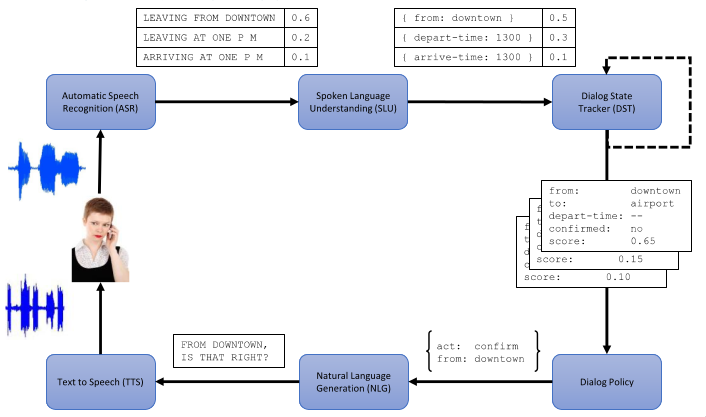
\includegraphics[scale=0.6]{07/sd.png}
    \caption{Componenti di un sistema di dialogo.}
\end{figure}

\paragraph{Un sistema di dialogo ha:}

\begin{itemize}
  \item \fancyglitter{NLU:} riempe i buchi usando le risposte dell'utente.
  \item \fancyglitter{NLG:} profuce testi più naturali, meno simili a dei template. 
  \item \fancyglitter{Tracker dello stato del dialogo:} mantiene lo stato corrente del dialogo.
  \item \fancyglitter{Politica di dialogo:} decide cosa il sistema debba fare o dire successivamente: 
    \begin{itemize}
      \item GUS policy: chiede domande finché non riesce a riempire il suo frame. 
      \item Politiche più complicate.
    \end{itemize}
\end{itemize}

\paragraph{Natural Language Understanding (NLU):}

\begin{itemize}
  \item Classico: 
    \begin{itemize}
      \item Significato = Sintassi $\rightarrow$ Semantica $\rightarrow$ Pragmatica.
    \end{itemize}
  \item Moderno (più usato nei Dialog Systems): 
    \begin{itemize}
      \item Semantica più semplice: GUS Slot. 
      \item Assume una semantica a frames.
    \end{itemize}
\end{itemize}

\dfn{Agenti di Dialogo Basati sui Frames}{
  Sono sistemi che hanno come goal l'aiutare l'utente a risolvere un task come effettuare una prenotazione o comprare un prodotto.
}

\nt{A volte sono chiamati agenti di dialogo basati su tasks.}

\dfn{GUS}{Il primo sistema proposto fu GUS (1977): una struttura rappresentante le intenzioni degli utenti. Era composta da uno o più frame ognuno con slots e valori.}

\paragraph{Algoritmo di GUS:}

\begin{enumerate}
  \item Rilevamento del dominio $\rightarrow$ Insieme di frames. 
  \item Rilevamento delle intenzioni $\rightarrow$ Un frame.
  \item Riempimento di uno slot $\rightarrow$ Riempimento di un frame.
\end{enumerate}

\cor{Frame}{
  Un insieme di slots che devono essere riempiti con informazioni di un determinato tipo. Ognuno è associato a una domanda posta all'utente.
}

\nt{A volte un frame è chiamato ontologia del dominio.}

\paragraph{Struttura di controllo per GUS:}

\begin{itemize}
  \item Il sistema fa domande all'utente, riempendo specifici slots.
  \item Si possono riempire più slots contemporaneamente. 
  \item Quando un frame è pieno si fa una query sul database.
  \item Il tutto termina quando si sono riempiti tutti i buchi.
  \item Il sistema deve capire quale slot di quale frame riempire. 
\end{itemize}

\paragraph{Come si capisce quale slot riempire?}

\begin{itemize}
  \item Classificazione del dominio. 
  \item Determinare le intenzioni. 
  \item Riempire lo slot.
\end{itemize}

\paragraph{Problemi con i frames:}

\begin{itemize}
  \item Non sono facilmente applicabili a tasks complessi: 
    \begin{itemize}
      \item Alcune informazioni potrebbero essere relative a più frames. 
      \item Ricorsività. 
    \end{itemize}
  \item Frames complessi: 
    \begin{itemize}
      \item Si costruisce una gerarchia di frame. 
    \end{itemize}
\end{itemize}

\nt{Si possono avere sistemi ibridi con frames e apprendimento.}

\section{Valutazione}

\qs{}{Come si valuta la bontà di un sistema di dialogo o di un ChatBOTs?}

\begin{itemize}
  \item ChatBOTs: tramite interazioni con gli utenti. 
  \item Dialoghi task-based: misurando le performance dei tasks.
\end{itemize}

\subsection{Trindi Tricklist}

\begin{enumerate}
  \item L'interpretazione è relativa al contesto?
  \item Il sistema può gestire risposte che forniscono più informazioni di quelle richieste?
  \item Il sistema può gestire risposte che forniscono informazioni diverse da quelle attese?
  \item Il sistema può gestire risposte che forniscono meno informazioni di quelle richieste? 
  \item Il sistema può gestire risposte ambigue? 
  \item Il sistema può gestire negazioni? 
  \item Il sistema può gestire l'assenza di risposta? 
  \item Il sistema può gestire input contenenti "rumore"? 
  \item Il sistema può gestire sotto-dialoghi iniziati dall'utente? 
  \item Il sistema chiede solo domande adeguate? 
  \item Il sistema può gestire informazioni inconsistenti? 
  \item Il sistema può gestire una revisione delle credenze\footnote{Meglio visto nel corso di "Agenti Intelligenti".}? 
  \item Il sistema controlla la sua comprensione delle intenzioni dell'utente?
\end{enumerate}







